\ifx\allfiles\undefined
\documentclass[12pt, a4paper,oneside, UTF8]{ctexbook}
\usepackage[dvipsnames]{xcolor}
\usepackage{amsmath}   % 数学公式
\usepackage{amsthm}    % 定理环境
\usepackage{amssymb}   % 更多公式符号
\usepackage{graphicx}  % 插图
\usepackage{mathrsfs}  % 数学字体
\usepackage{enumitem}  % 列表
\usepackage{geometry}  % 页面调整
\usepackage{unicode-math}
\usepackage[colorlinks,linkcolor=blue,anchorcolor=blue,citecolor=blue]{hyperref}
\usepackage{tcolorbox}
\usepackage{subfigure}
\usepackage{utfsym}
\usepackage{bm}
\usepackage{diagbox}
\usepackage{tabularx}
\usepackage[]{algorithm, algorithmicx, algpseudocode}
\usepackage{framed}
\tcbuselibrary{most}
\usepackage[]{bm}
\graphicspath{ {img/},{../img/}, {img/}, {../img/} }  % 配置图形文件检索目录
\linespread{1.5} % 行高

% 页码设置
\geometry{top=25.4mm,bottom=25.4mm,left=20mm,right=20mm,headheight=2.17cm,headsep=4mm,footskip=12mm}

% 设置列表环境的上下间距
\setenumerate[1]{itemsep=5pt,partopsep=0pt,parsep=\parskip,topsep=5pt}
\setitemize[1]{itemsep=5pt,partopsep=0pt,parsep=\parskip,topsep=5pt}
\setdescription{itemsep=5pt,partopsep=0pt,parsep=\parskip,topsep=5pt}

% 定理环境
% ########## 定理环境 start ####################################
% #### 将 config.tex 中的定理环境的对应部分替换为如下内容
% 定义单独编号,其他四个共用一个编号计数 这里只列举了五种,其他可类似定义(未定义的使用原来的也可)
\newtcbtheorem[number within=section]{defn}%
{Def.}{colback=OliveGreen!10,colframe=Green!70,fonttitle=\bfseries}{def}

\newtcbtheorem[number within=section]{lemma}%
{Lemma}{colback=Salmon!20,colframe=Salmon!90!Black,fonttitle=\bfseries}{lem}

% 使用另一个计数器 use counter from=lemma
\newtcbtheorem[use counter from=lemma, number within=section]{them}%
{Theorem}{colback=SeaGreen!10!CornflowerBlue!10,colframe=RoyalPurple!55!Aquamarine!100!,fonttitle=\bfseries}{them}

\newtcbtheorem[use counter from=lemma, number within=section]{recall}%
{Recall}{colback=green!5,colframe=green!35!black,fonttitle=\bfseries}{rel}

\newtcbtheorem[use counter from=lemma, number within=section]{remark}%
{Remark}{colback=Emerald!10,colframe=cyan!40!black,fonttitle=\bfseries}{remark}
% colback=red!5,colframe=red!75!black

% 这个颜色我不喜欢
\newtcbtheorem[number within=section]{Notes}%
{Notes}{colback=red!5,colframe=red!75!black,fonttitle=\bfseries}{notes}

\newtcbtheorem[number within=section]{Properties}%
{Properties}{colback=blue!5,colframe=blue!75!black,fonttitle=\bfseries}{Properties}

\newtcbtheorem[number within=section]{Examples}%
{Examples}{colback=red!5,colframe=red!45!black,fonttitle=\bfseries}{Examples}
% .... 命题 例 注 证明 解 使用之前的就可以(全文都是这种框框就很丑了),也可以按照上述定义 ...
% 两种方式定义中文的 证明 和 解 的环境:
% 缺点:\qedhere 命令将会失效【技术有限,暂时无法解决】
\renewenvironment{proof}{\par\textbf{证明.}\;}{\qed\par}
\newenvironment{solution}{\par{\textbf{解.}}\;}{\qed\par}

% 缺点:\bf 是过时命令,可以用 textb f等替代,但编译会有关于字体的警告,不过不影响使用【技术有限,暂时无法解决】
%\renewcommand{\proofname}{\indent\bf 证明}
%\newenvironment{solution}{\begin{proof}[\indent\bf 解]}{\end{proof}}
% ######### 定理环境 end  #####################################

% ↓↓↓↓↓↓↓↓↓↓↓↓↓↓↓↓↓ 以下是自定义的命令  ↓↓↓↓↓↓↓↓↓↓↓↓↓↓↓↓

% 用于调整表格的高度  使用 \hline\xrowht{25pt}
\newcommand{\xrowht}[2][0]{\addstackgap[.5\dimexpr#2\relax]{\vphantom{#1}}}

% 表格环境内长内容换行
\newcommand{\tabincell}[2]{\begin{tabular}{@{}#1@{}}#2\end{tabular}}

% 使用\linespread{1.5} 之后 cases 环境的行高也会改变,重新定义一个 ca 环境可以自动控制 cases 环境行高
\newenvironment{ca}[1][1]{\linespread{#1} \selectfont \begin{cases}}{\end{cases}}
% 和上面一样
\newenvironment{vx}[1][1]{\linespread{#1} \selectfont \begin{vmatrix}}{\end{vmatrix}}

\def\d{\textup{d}} % 直立体 d 用于微分符号 dx
\def\R{\mathbb{R}} % 实数域
\def\K{\mathcal{K}} % any set representation used in definition
\newcommand{\bs}[1]{\boldsymbol{#1}}    % 加粗,常用于向量
\newcommand{\ora}[1]{\overrightarrow{#1}} % 向量

% 数学 平行 符号
\newcommand{\pll}{\kern 0.56em/\kern -0.8em /\kern 0.56em}

% 用于空行\myspace{1} 表示空一行 填 2 表示空两行  
\newcommand{\myspace}[1]{\par\vspace{#1\baselineskip}}

%%%%cite url link%%%%%%%%%
\usepackage{url}

%%%%%%%%%%%%%%%%%%%

%%%%%%% Custom Command %%%%%%%
\renewcommand{\thefootnote}{\arabic{footnote}}

%%%%%%%%%%%%%%%%%%%
\begin{document}
	% \title{{\Huge{\textbf{Convex Optimization Note}}}}
\author{Zelin Yao}
\date{\today}
\maketitle                   % 在单独的标题页上生成一个标题

\thispagestyle{empty}        % 前言页面不使用页码
\begin{center}
	\Huge\textbf{前言}
\end{center}

if people do not believe that mathematics is simple, 
it is only because they do not realize how complicated life is. ——John von Neumann

\begin{flushright}
	\begin{tabular}{c}
		\today \\ 与其焦虑不如先行动起来!
	\end{tabular}
\end{flushright}

\newpage                      % 新的一页
\pagestyle{plain}             % 设置页眉和页脚的排版方式(plain:页眉是空的,页脚只包含一个居中的页码)
\setcounter{page}{1}          % 重新定义页码从第一页开始
\pagenumbering{Roman}         % 使用大写的罗马数字作为页码
\tableofcontents              % 生成目录

\newpage                      % 以下是正文
\pagestyle{plain}
\setcounter{page}{1}          % 使用阿拉伯数字作为页码
\pagenumbering{arabic}
% \setcounter{chapter}{-1}    % 设置 -1 可作为第零章绪论从第零章开始 % 单独编译时,其实不用编译封面目录之类的,如需要不注释这句即可
	\else
	\fi
	%  ↓↓↓↓↓↓↓↓↓↓↓↓↓↓↓↓↓↓↓↓↓↓↓↓↓↓↓↓ 正文部分
	\chapter{Optimization Basis}
	\section{KKT Conditions}

	\section{Derivatives}
	This note is summarized by \cite{directionalderivatievesandthegradientvector}.
	
	Consider a function $f:\R^n \rightarrow \R$,  \emph{the partial derivatives, directional derivatives} have the following definitions,
	\begin{defn}{Partial Derivatives, Directional Derivatives}{}
	Assume $e_i$ is the unit vector in the $x_i$ direction, the \emph{partial derivative} of function $f(\vec x)$ in the $x_i$ direction is,
	$$
	\frac{\partial f(\vec x)}{\partial x_i} = \lim_{\alpha\rightarrow 0}\frac{f(\vec x+\alpha e_i)-f(\vec x)}{\alpha}
	$$
	The \emph{directional derivative} of $f(\vec x)$ in direction $d$ is,
	$$
	f^{'}(\vec x;d) =  \lim_{\alpha\rightarrow 0}\frac{f(\vec x+\alpha d)-f(\vec x)}{\alpha}
	$$
	If the function $f(\vec x)$ is differentiable of each directions, and the direction $d$ is a \textbf{unit vector}, the following relation is satisfied,
	$$
	f^{'}(\vec x;d) = \sum_{i=1}^n \frac{\partial f(\vec x)}{\partial x_i} d_i = [\frac{\partial f(\vec x)}{\partial x_i}]_{i\in[n]}^Td=\nabla f(\vec x)^Td
	$$
	If we check the the directional derivative of function $f(x,y,z) = y^2d^{xyz}$ in direction $d=(0,1,2)$ and the gradient, the unit vector of the direction is necessary.
	\end{defn}
	
	\section{Matrix Calculus}
	If the variables about domains are considered as inputs of a system, and the variables about ranges are called outputs of a system, these inputs and outputs can be divided into three types, i.e. scalars, vectors, and matrices. 
	\textbf{This article is based on \emph{Numerator Layout}, whose means will demonstrate as following!}
	This table can clearly describe all situations.
	 \begin{table}[!htp]
		\centering
		\caption{The Types of All Derivatives} 
		\begin{tabular}{l|l|l|l}
			\hline
			\diagbox{Output}{Input}& Scalar  & Vector & Matrix \\
			\hline
			Scalar & $f^{'}(x)$ & $f(\vec x):\R^{m\times 1}\rightarrow \R$ & $f(X):\R^{m\times n}\rightarrow \R$ \\
			\hline
			Vector & $\vec f(x):\R\rightarrow \R^{m\times 1}$ & $\vec f(\vec x):\R^{m\times 1}\rightarrow \R^{n\times 1}$ & $\vec f(X):\R^{m\times n}\rightarrow \R^{n\times 1}$ \\
			\hline
			Matrix & $F(x):\R\rightarrow \R^{m\times n}$ & $F(\vec x):\R^{m\times 1}\rightarrow \R^{p\times q}$ & $F(X):\R^{m\times n}\rightarrow \R^{p\times q}$ \\
			\hline
		\end{tabular}
	\end{table}
	In optimization problem, the most common situations are scalar output, and learning it is critical!
	
	\begin{Notes}{The Meaning of \emph{Numerator Layout} and \emph{Denominator Layout}}{} \label{Notes 1}
		Firstly, considering a function $\vec f (\vec x):\R^{n\times 1}\rightarrow \R^{m\times 1}$, which means that the input and output are both vector and not matrices. If its derivative is arranged as following and the dimension of each elements is equal to the numerator of derivative, we call this layout to be \emph{Numerator Layout}. The results of \emph{Denominator Layout} is just the transpose of the results of \emph{Numerator Layout}. 
		
		We first construct the \textbf{outer matrix}, which decomposes the vector $\vec x$ to $x_1,x_2,...,x_n$ and forms derivatives by ${\partial \vec f (\vec x)}/{\partial x_i},\forall i \in \{1,2,...,n\}$. And more important, the dimension of \textbf{outer matrix} is equal to the dimension of transposed denominator.
		$$
		\frac{\partial \vec f (\vec x)}{\partial \vec x}=\begin{pmatrix} {\partial \vec f (\vec x)}/{\partial  x_1} & {\partial \vec f (\vec x)}/{\partial x_2} & ... & {\partial \vec f (\vec x)}/{\partial x_n}\end{pmatrix}
		$$
		Each elements is called \textbf{inner matrix}, which has the following form,
		$$
		\frac{\partial \vec f (\vec x)}{\partial x_i} = \begin{pmatrix} {\partial f_1 (\vec x)}/{\partial  x_i} \\ {\partial f_2 (\vec x)}/{\partial x_i}\\ ... \\ {\partial f_m (\vec x)}/{\partial x_i}\end{pmatrix}
		\in \R^{m\times 1}$$
	\end{Notes}

	\subsection{Notation}
		
	\subsection{Basic Methods}
		\textbf{Method Based on Elements} \\
		 \par This method uses the definition of \fbox{Note \ref{Notes 1}}. The key of this method is that based on single input and output problem decomposing other problems into single variable problem. Next we give some examples in \fbox{subsection \ref{subsection_examples}}. Actually, this method can be used to prove some theorems or formulation, but it is costly.\\
		 
		 \textbf{Method Based on Limitation}\\
		 \par Firstly, recall the differential of $f(x)$ that is \textbf{scalar input and scalar output}. The difference (not differential) has this form,
		 $$
		 \Delta f = f(x+\Delta x)-f(x) = f^{'}(x)\Delta x + o(||\Delta x||)
		 $$
		 Let $\Delta x\rightarrow 0$. The $\Delta x$ is transformed to $dx$ (maybe mathematical abuse), and high-order term is omitted. The \emph{differential} can be reformulated as,
		 $$
		 df = f(x+dx)-f(x) = f^{'}(x)dx
		 $$
		 In this time, the simplest situation is solved, but how we know the definition of gradient and etc.\\
		 \par Secondly, some other situations about scalar and vector (the situations about matrices are a little bit different) are considered. According to the definition of scalar input and scalar output, the situation of \textbf{vector input and scalar output} is similar. \\
		 Consider $f(\vec x):\R^{n}\rightarrow \R$. Similar with the situation of scalar input and scalar output, we have,
		 $$
		 df=f(\vec x+d\vec x)-f(\vec x)=f^{'}(\vec x)d\vec x
		 $$
		 In fact, the $f^{'}(\vec x)$ is called \emph{derivative} and it is a row vector (or covector/dual vector). The reason why it is a row vector is that the dimension match that $df$ belongs to $\R$ and $d\vec x$ is a column vector. Obvious, the result is in line with the definition by elements. The \textbf{\emph{gradient}} is the transposed derivative. \\
		 The situation of \textbf{scalar input and vector output} is similar with the situation of vector input and scalar output. The difference between them is the dimension of derivative (actually the relation of transposing).\\
		 The most critical situation is \textbf{vector input and vector output}. Using the definition by elements, the dimension of derivative is not obvious and the calculation is complex and trivial. But the method based on limitation can deal with it. Consider $\vec f(\vec x):\R^{n\times 1}\rightarrow \R^{m \times 1}$. The similar formulation is,
		 $$
		 	d\vec f = \vec f(\vec x+d\vec x) -\vec f(\vec x) = Jd\vec x
		 $$
		 Where $J\in\R^{m\times n}$ to match dimension of $d\vec f$ and $d\vec x$.\\
		 
		 \par Thirdly, the special and critical situations are the input or output associated matrices. \textbf{The differential can be represented as the dot product of derivative and $dX$, but if the input or output is matrix, the dot product of matrix must be defined again to make the situation satisfy the definition of scalar and vector situation.} A new dot product definition will be introduced, and trace and vec are used to simplify expressions. New definition about dot product is defined as following.
		 \begin{defn}{The Definition of Matrices Dot Product}{}
		 	The meaning of dot product is the sum of multiplying all corresponding elements. The \emph{dot product} of matrix $A$ and $B$ is that
		 	\begin{equation*}
		 	\begin{split}
			 	A\bullet B&= \sum_{i}\sum_{j}A_{ij}B_{ij}\\
			 	&=\langle A,B\rangle \\
			 	&=vec(A)^Tvec(B) \\
			 	&=tr(A^TB)\\
			 	&=tr(BA^T)
		 	\end{split}
	 		\end{equation*}
		 \end{defn}
	 	
	 	The detailed examples about matrices are shown in \fbox{subsection \ref{subsection_examples}}
	 
	\subsection{Derivative Properties and Other Prerequisites}
		\textbf{These properties is useful to the all situation whatever scalars, vectors and matrices. And \emph{Numerator Layout} is adapted.} I will list all of them, and proof some important theorems in \fbox{subsection \ref{subsection_examples}}.
		
		\begin{Properties}{Derivative Properties}{}
			
			\begin{enumerate}
				\item \textbf{(Sum Rule)} if $f(x)=g(x)+h(x);f,g,h$ are scalar, vector, or matrix function, then $df=dg+dh$ and $df/dx=dg/dx+dh/dx$
				\item \textbf{(Product Rule)}if $f(x)=g(x)h(x);f,g,h$ are scalar, vector, or matrix function, then $df=dgh+gdh$. Notice that the order cannot be changed!
				\item \textbf{(Chain Rule)}if $f(x)=g(h(x));f,g,h$ are scalar, vector, or matrix function, then $df=dg(h(x))dh(x)$. Another equivalent formulation is that $\frac{df}{dx}=\frac{dg(h(x))}{dh(x)}\frac{dh(x)}{dx}$. Using method of elements to prove it easily. 
				
				Notice that the order cannot be changed!
				\item \textbf{(Linearity)} $d(au(x)+bv(x))/{dx} =d(u(x))/dx+d(v(x))/dx$. We have proofed this property is satisfied when \underline{scalar/vector/matrix input} and \underline{scalar/vector/matrix output}.
			\end{enumerate}
		Their proofs are convenient when using the method of elements.
		\end{Properties}
	
		\begin{Properties}{Trace}{}
			\begin{enumerate}
				\item (Linearity) Assume $a,b$ are constant, $A,B$ are same dimensional matrices. $tr(aA\pm bB)=atr(A)+btr(B)$
				\item (Transpose) $tr(A) = tr(A^T)$
				\item (Matrix Dot Product) $tr(A^TB)=tr(B^TA)=tr(AB^T)=tr(BA^T)=\langle A,B\rangle = \sum_{i}\sum_{j}A_{ij}B_{ij}$
				\item (Cyclic Property) Assume three asymmetric matrices $A,B,C$ $\Rightarrow tr(ABC)=tr(BCA)=tr(CAB)$. Assume three symmetric matrices $A,B,C$, the order in trace can be changed arbitrarily.
			\end{enumerate}
		\end{Properties}
	
		\begin{Properties}{Kronecker Product}{}
			
			\begin{enumerate}
				\item (Trace) Assume $A,B$ are symmetric, and then $tr(A\otimes B)=tr(A)tr(B)$.
				\item (Transpose and Inverse) $(A\otimes B)^T=(A^T)\otimes(B^T)$ and $(A\otimes B)^{-1}=(A^{-1})\otimes(B^{-1})$. Under Kronecker Product, the inverse and transpose cannot change the multiple order.
				\item (Kronecker Sum/Tensor Sum) Assume $A\in \R^{n\times n},B\in \R^{m\times m}$, $A\oplus B=(I_m\otimes A)+(B\otimes I_n)\in\R^{mn\times mn}$
				\item (vec/span a matrix column by column) $vec(ABC)=(C^T\otimes A)vec(B)$ for any matrix $A,B,C$.
			\end{enumerate}
		\end{Properties}
	
	\subsection{Some Examples, Proofs and Applications} \label{subsection_examples}
		\subsubsection{$\mathbf{f(x):\R\rightarrow\R}$}
			Easy!
		\subsubsection{$\mathbf{f(x):\R^{m\times 1}\rightarrow\R}$}
			\begin{Examples}{}{}
				1. $f(\vec x)=\vec x^TA\vec x,x\in \R^{m\times1},A\in\R^{m\times m}$. \\
				\underline{Sol1:} (Method of elements)Firstly, the outer matrix can be written as,
				$$\frac{\partial f(\vec x)}{\partial x}=\begin{pmatrix}\partial f(\vec x)/\partial x_1,...,\partial f(\vec x)/\partial x_m \end{pmatrix}$$
				where the dimension of outer matrix is the dimension of transposed denominator. Then each inner matrices can be expressed as,
				$$
				\frac{\partial f(\vec x)}{\partial x_i}=2A_{ii}x_i+\sum_{k\neq i}(A_{ki}+A_{ik})x_k=\sum_{k=1}^{m}(A_{ki}+A_{ik})x_k
				$$
				So, substitute the elements of outer matrix with inner matrix, then the derivative is
				$$
				\frac{\partial \vec x^TA\vec x}{\partial \vec x}=x^T(A+A^T)
				$$
				
				\underline{Sol2:}(Method based on limitation) The method of elements is trivial. But if we use the properties of derivative fully, the situation will be easy to tackle.
				\begin{equation*}
				\begin{split}
					df&=f(\vec x+d\vec x)-f(\vec x)\\
					&=(\vec x+d\vec x)^TA(\vec x+d\vec x)-\vec x^TA\vec x\\
					&=d\vec x^TA\vec x+\vec x^TAd\vec x+d\vec x^TAd\vec x
				\end{split}
				\end{equation*}
				Because this method is based on limitation and omits the notation of limit, the limitation of $d\vec x$can be expressed as $d\vec x\rightarrow 0$. So the above equation can be,
				\begin{equation*}
				\begin{split}
						df&=f(\vec x+d\vec x)-f(\vec x)\\
						&=d\vec x^TA\vec x+\vec x^TAd\vec x\\
						&=(d\vec x^TA\vec x)^T +\vec x^TAd\vec x\quad \quad \text{\textbf{the transpose of scalar is still this scalar}}\\
						&=\vec x^T(A+A^T)d\vec x
				\end{split}
				\end{equation*}
				So the derivative of the given function is $\vec x^T(A+A^T)$, and the gradient is $(A+A^T)\vec x$
				
				\underline{Sol3:}(Derivative properties) $df=d\vec x^TA\vec x+\vec x^TdA\vec x+\vec x^TAd\vec x$. Transform it, and the result is obvious.
 			\end{Examples}
 		
 			\begin{Examples}{$l2-norm$}{}
 				$f(\vec x)=||\vec x||_2,\vec x\in\R^{m\times1}$\\
 				Squaring both sides,
 				$$f(\vec x)f(\vec x)=||\vec x||_2^2=\vec x^T\vec x$$ \\
 				Using derivative properties,
 				$$2fdf=d\vec x^T\vec x+\vec x^Td\vec x=2\vec x^Td\vec x$$
 				So the derivative of $f$ is,
 				$$
 				df(\vec x) = \frac{\vec x^T}{f(\vec x)}d\vec x=\frac{\vec x^T}{||\vec x||_2}d\vec x
 				$$
 				All in all, the derivative of $l2-norm$ is $\frac{\vec x^T}{||\vec x||_2}$, and the gradient is $\frac{\vec x}{||\vec x||_2}$
 			\end{Examples}
 		
		\subsubsection{$\mathbf{f(x):\R^{m\times n}\rightarrow\R}$}
			\begin{Examples}{Inverse}{}
				$f(X)=X^{-1},X\in\R^{m\times m}\rightarrow \R$\\
				In fact, the method based on limitation and derivative properties is effective in calculating derivative, but not useful in proof. We have,
				$$X^{-1}X=I$$
				By product rule of derivative, we have,
				$$dX^{-1}X+X^{-1}dX=dI=0$$
				So, the derivative of the inverse of $X$ is,
				$$dX^{-1}=-X^{-1}dXX^{-1}$$
			\end{Examples}
			
			\begin{Examples}{$F-norm$}{}
				$f(X)=||X||_F=\sqrt{tr(X^TX)},X\in\R^{m\times n}\rightarrow \R$\\
				Firstly, using chain rule of derivative,
				$$
				df(X) = \frac{d(tr(X^TX))}{2\sqrt{tr(X^TX)}}
				$$
				According to the property of trace ($d(tr(A))=tr(d(A))$),
				\begin{equation*}
				\begin{split}
				df(X) &= \frac{tr(d(X^TX))}{2\sqrt{tr(X^TX)}}\\
				&= \frac{tr(d(X^T)X))}{2\sqrt{tr(X^TX)}}+\frac{tr(X^TdX))}{2\sqrt{tr(X^TX)}}
				\end{split}
				\end{equation*}
				Use the property of trace ($d(A^T)=d(A)$),
				\begin{equation*}
					\begin{split}
						df(X) &= \frac{tr(X^TdX))}{\sqrt{tr(X^TX)}}\\
						&=\frac{X\bullet dX}{||X||_F} \quad \quad \text{\textbf{(The definition of matrix dot product)}}					
					\end{split}
				\end{equation*}
				So, the derivative of $||X||_F$ is $X/||X||_F$, and the gradient is $X^T/||X||_F$
			\end{Examples}
		
			\begin{Examples}{Determinant}{}
				$f(X)=det(X),X\in\R^{m\times m}\rightarrow \R$\\
				Without doubt, the method based on limitation is used.
				\begin{equation*}
				\begin{split}
					df(X) &= det(X+dX)-det(X) \\
					&=det(X+XX^{-1}dX)-det(X) \\
					&=det(X(I+X^{-1}dX))-det(X) \\
					&=det(X)det(I+X^{-1}dX) -det(X)
				\end{split}
				\end{equation*}
				The determinant can be treated as the multiplication of eigenvalues. Assume the eigenvalues of $X^{-1}dX$ are $\lambda_1,\lambda_2,...,\lambda_m$, the eigenvalues of $I+X^{-1}dX$ are $1+\lambda_1,1+\lambda_2,...,1+\lambda_m$. So the deternimant of $I+X^{-1}dX$ is,
				\begin{equation*}
					\begin{split}
						det(I+X^{-1}dX)&=(1+\lambda_1)(1+\lambda_2)...(1+\lambda_m) \\
						&=1+(\lambda_1+\lambda_2+...+\lambda_m)+...\\
						&\approx 1+(\lambda_1+\lambda_2+...+\lambda_m)
					\end{split}
				\end{equation*}
				So, $det(X)=det(X)(\lambda_1+\lambda_2+...+\lambda_m)=tr(det(X)X^{-1}dX)$
			\end{Examples}
		
		\subsubsection{$\mathbf{f(x):\R^{m\times 1}\rightarrow\R^{n\times1}}$}
			\begin{Examples}{}{}
				$\vec f(\vec x)=A\vec x,A\in\R^{m\times n}\rightarrow \R^{v\times1}$\\
				Similarly, using the method of elements is complex. We use properties and limitation here to solve it.
				$$
				d\vec f=dA\vec x+Ad\vec x=Ad\vec x
				$$
				The derivative is $A$, and the gradient is $A^T$.
			\end{Examples}
		
		\subsubsection{$\mathbf{f(x):\R^{m\times n}\rightarrow\R^{p\times q}}$}
		\begin{Examples}{}{}
			$F(X)=X^3,X\in\R^{m\times m}\rightarrow \R^{m\times m}$\\
			Briefly writing the process,
			$$
			dF = dXX^2+XdXX+X^2dX
			$$
			Meet some problems that the $dF$ cannot be represented the explicit form of $(\cdot) \bullet dX$. But if the new notation of $vec$ (span a matrix column by column and link with them)is used, the problem is solved. According to the property of $vec(ABC)=(C^T\otimes A)vec(B)$,
			\begin{equation*}
			\begin{split}
			&vec(dF)=vec(dXX^2)+vec(XdXX)+vec(X^2dX) \\
			\Leftrightarrow& vec(dF)=vec(IdXX^2)+vec(XdXX)+vec(X^2dXI) \\
			\Leftrightarrow& vec(dF)=(X^2\otimes I)vec(dX)+(X\otimes X)vec(dX)+(I\otimes X^2)vec(dX) \\
			\Leftrightarrow& vec(dF)=((X^2\otimes I)+(X\otimes X)+(I\otimes X^2))vec(dX) \\
			\end{split}
			\end{equation*}
		\end{Examples}
	
	\section{Random Vectors, Random Matrices, and Their Expected Values }
	This note comes from the summary of  \href{http://www.statpower.net/Content/313/Lecture\%20Notes/MatrixExpectedValue.pdf}{James H. Steiger}. 
	
	Some intuitive senses,
	\begin{enumerate}
		\item \emph{random vectors} or \emph{random matrices} are these vectors or matrices that each of their elements is a single random variable.
		\item The expectation of random vector is vector that expects its all elements.
	\end{enumerate} 
	
	
	
	\section{Convexity and Smoothness} 
	The definition and some explanations are stemmed form \cite{hazan2023introductiononlineconvexoptimization}, \cite{gormley2023introductiononlineconvexoptimization}, \cite{aaron2017convexity}.
		\begin{defn}{Convexity}{}
			1. A \emph{set} $\mathcal{K}$ is convex if $\forall x,y\in \mathcal{K}$, $\alpha\in [0,1]$, we have $\alpha x+(1-\alpha)y\in \mathcal{K}$ \\
			2. A \emph{function} $f:\mathcal{K}\rightarrow \R$ is convex if $\forall x,y\in \mathcal{K}$, $\alpha\in [0,1]$, we have $f(\alpha x+(1-\alpha)y)\le \alpha f(x)+(1-\alpha)f(y)$ \\
			3. A \emph{differentiable function} $f:\mathcal{K}\rightarrow \R$ is convex if and only if  $\forall x,y\in \mathcal{K}$, we have $f(y)\ge f(x)+\nabla f(x)^T(y-x)$
		\end{defn}
	
		\begin{defn}{$\alpha$-strongly Convex}{}
			1. A \emph{function} $f$ is $\alpha$-strongly convex if $\forall x,y\in \mathcal{K}$, we have $ f(y)\ge f(x)+\nabla f(x)^T(y-x)+\frac{\alpha}{2}||y-x||^2$ or $||\nabla f(x)-\nabla f(y)||\ge \alpha ||x-y||$ or $f(x)-\frac{\alpha}{2}||x||^2$ is convex.\\
			2. A \emph{twice differentiable function} $f$ is $\alpha$-strongly convex if $\nabla^2 f(x)\succeq \alpha I$\\
			
		\end{defn}
		
		\begin{defn}{$\beta$-smooth}{}
			1. A \emph{function} $f$ is $\beta$-smooth if $\forall x,y\in \mathcal{K}$, we have $ f(y)\le f(x)+\nabla f(x)^T(y-x)+\frac{\beta}{2}||y-x||^2$ or $||\nabla f(x)-\nabla f(y)||\le \beta ||x-y||$. \\
			2. A \emph{twice differentiable function} $f$ is $\beta$-smooth if $\nabla^2 f(x) \preceq \beta I$\\
			3. If $f$ is $\beta$-smooth then $\frac{\beta}{2}||x||^2-f(x)$ is convex.
		\end{defn}
		 
		 The \emph{condition number} of a $\gamma$-well-conditioned function is defined to be the ratio between strong convexity and smoothness.
		 $$
		 \gamma = \frac{\alpha}{\beta} \le1
		 $$
		 $ f(y)\ge f(x)+\nabla f(x)^T(y-x)+\frac{\alpha}{2}||y-x||^2$ can be interpreted as fixing a point $x$. The part of $f(x)+\nabla f(x)^T(y-x)$ is the linear part or tangent of the function $f(x)$ at point $x$. This inequality shows that the curve of $f(y)$ is \emph{above} the tangent plus a parabola. The analysis of smooth is similar.
		 
		 \begin{Properties}{The Properties of Convexity and Smoothness}{}
		 	\begin{enumerate}
			 	\item If $f_1$ is a $\alpha_1$-strongly convex, $f_2$ is a $\alpha_2$-strongly convex. Then $f_1+f_2$ is ($\alpha_1+\alpha_2$)-strongly convex in $dom(f_1)\cap dom(f_2)$. 
			 	\item If $f_1$ is a $\beta_1$-smooth, $f_2$ is a $\beta_2$-smooth. Then $f_1+f_2$ is ($\beta_1+\beta_2$)-smooth in $dom(f_1)\cap dom(f_2)$.
			 	\item \textbf{The function $\frac{\alpha}{2}||x-x_1||^2_2$ is $\alpha$-strongly convex and $\alpha$-smooth.}
		 	\end{enumerate}
		 \end{Properties}
		 
	\section{Cones and Optimality Conditions} \label{Cones and Optimality Conditions}
	 This note comes from \fbox{Lecture 6} of \cite{gormley2023introductiononlineconvexoptimization}.
	 
	 There are two types of cones (\emph{normal cone} and \emph{tangent cone}) that are important to deduce optimality condition. And have to mention that sometimes the definition uses $x$ to represent vector and sometimes point. \underline{$x$ is a point in this note}.
	 
	 \begin{defn}{Normal Cone}{}
	 	Given any set $\mathcal{K}$ (\textbf{convex or not convex}), and a point $x\in \mathcal{K}$, the \emph{normal cone} of set $\mathcal{K}$ at point $x$ is defined as,
	 	$$
	 	\mathcal{N}_{\K}(x) =\{g \mid g^T(y-x)\le0, \forall y\in \mathcal{K}\}
	 	$$
	 \end{defn}
 		
 	 \begin{defn}{Tangent Cone (i.e. polar cone)}{}
 	 	Based on the definition of normal cone, the \emph{tangent cone} represents the set of feasible direction that walking along this direction is still possibly landing in set $\mathcal{K}$. Because the definition of normal cone is general including convex or non-convex, the definition of tangent cone is also do. 
 	 	
 	 	When $\K$ is a convex set, the \emph{tangent cone} is the polar of the normal cone and is a convex cone, and is defined as,
 	 	$$
 	 	T_{\K}(x) = \mathcal{N}_{\K}(x)^{\circ} = \{g\mid g^T(z-x)\le 0,\forall z\in\mathcal{N}_{\K}(X)\}
 	 	$$
 	 \end{defn}
	 \begin{figure}[htbp] \label{normal cone}
	 	\centering
	 	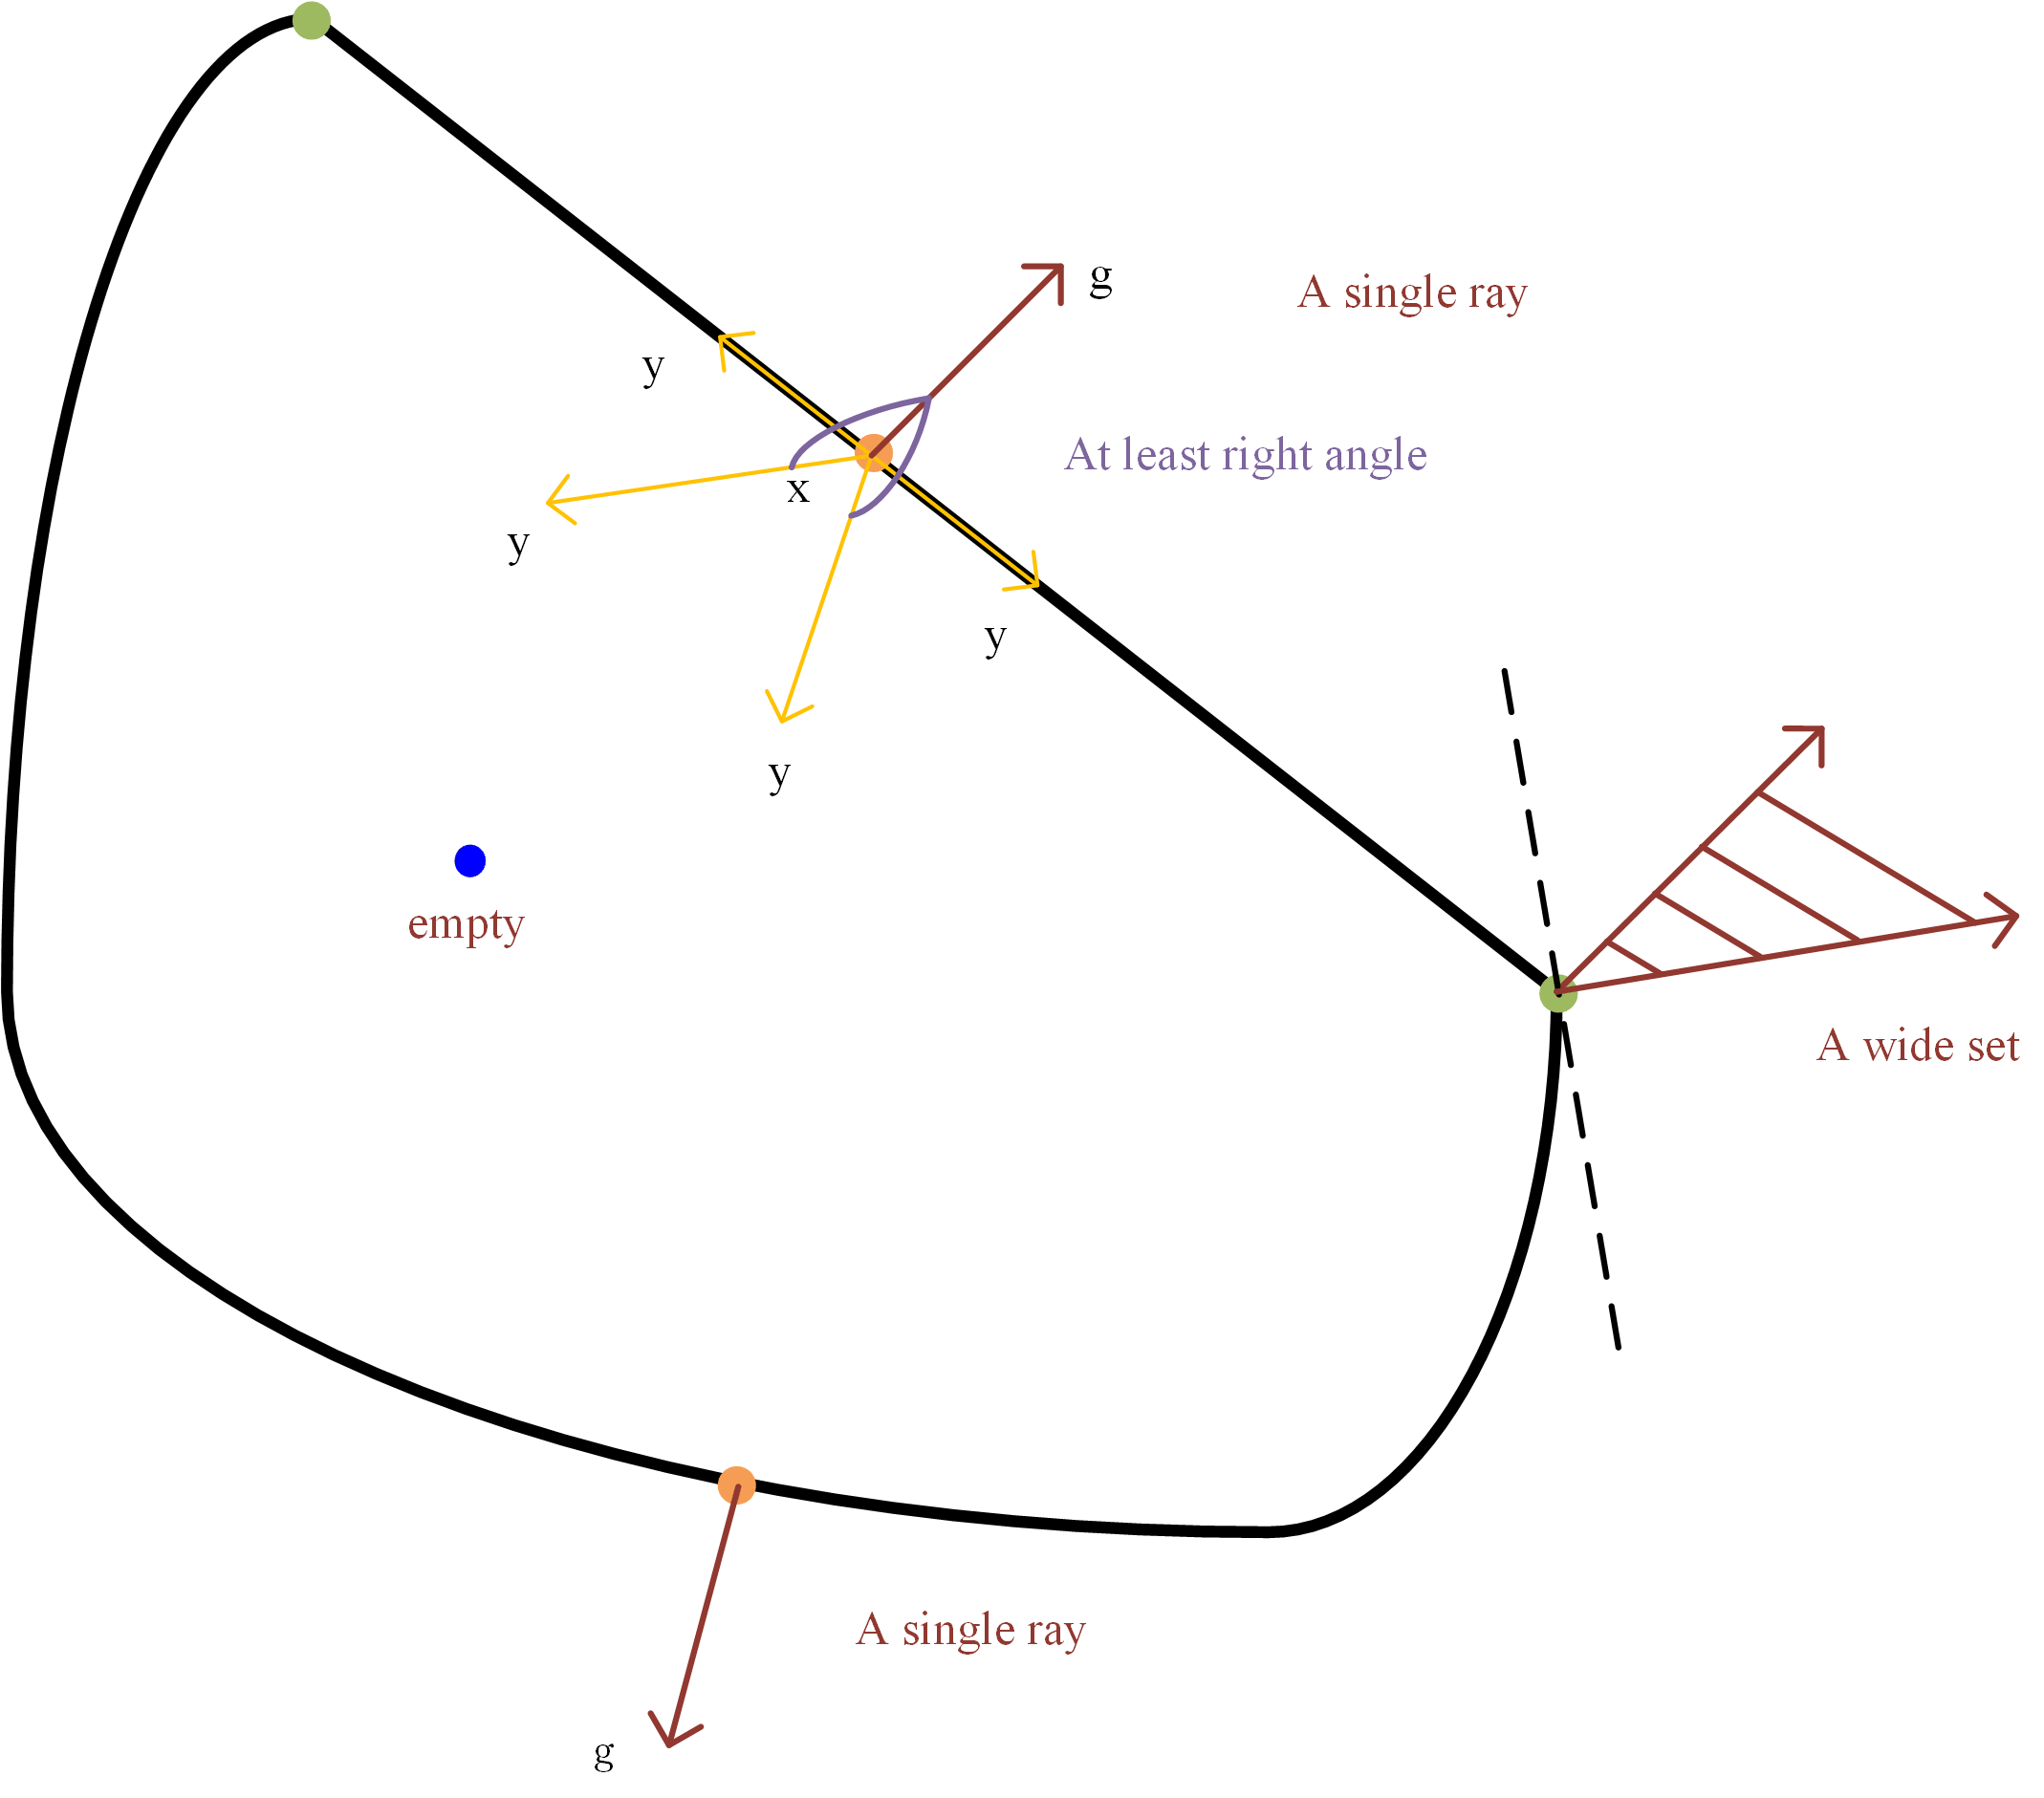
\includegraphics[scale=1]{img/normal_cone.png}
	 	\caption{The Explanation of Normal Cone}
	 \end{figure}
	 The normal cones at different points of set $\K$ is different, and can be classified into three cases.
	 \begin{enumerate}
	 	\item $x$ inside the set $\K$. The normal cone of it is empty, just as the \fbox{figure \ref{normal cone}} shown.
	 	\item $x$ at the boundary where it is smooth. The normal cone is a single ray, otherwise it does not satisfy at least right angle between $g$ and $(z-x)$.
	 	\item $x$ at the boundary where it is nonsmooth. This situation is a little bit complex. The all one-side tangents will be found, and the normal cone is the cone combined by these one-side tangents.
	 \end{enumerate}
	 
	 
	 \section{Optimality Conditions}
	 	This section will use the intuitive sense in \fbox{section\ref{Cones and Optimality Conditions}}.
	 	
	 	\textbf{Unconstrained Case} 
	 	\begin{enumerate}
	 		\item $x^*$ is optimal $\Leftrightarrow$ $0\in\partial f(x^*)$.
	 	\end{enumerate} 
	 	
	 	\textbf{Constrained Case}
	 	\begin{enumerate}
		 	\item $x^*$ is optimal $\Leftrightarrow$ $\nabla f(x^*)^T(y-x^*)\ge 0,\forall y\in \K$
		 	\item $x^*$ is optimal $\Leftrightarrow$ $-\nabla f(x^*)\in\mathcal{N}_{\K}(x^*)$ \quad \textbf{(by the definition of normal cone)}
	 	\end{enumerate}
	 	
	 	Under the constrained case, the gradient has three possible cases corresponding to the three cases of normal cone at different points.
	 	\begin{enumerate}
	 		\item $x^*$ inside the set $\K$. The minus gradient does not belong to $\mathcal{N}_{\K}(x^*)$,  because the normal cone is empty. And this problem degenerates to a unconstrained problem, using $\nabla f(x)=0$ to solve the minimum.
	 		\item $x^*$ at the boundary where it is smooth. The minus gradient is unique.
	 		\item $x^*$ at the boundary where it is nonsmooth. The minus gradient of optimal solution has a wide range.
	 	\end{enumerate}
 	
 	\section{Bregman Divergence}
 	This is a kind of method to measure distance, like metric. Bregman divergence is useful when analyzes the convergence rate about norm, because Bregman divergence can use some special properties to simplify proof.
 	\begin{defn}{Bregman Divergence}{}
 		Assume (a)$\Omega$ is a closed convex set, (b)function $f:\Omega\rightarrow\R$ is strictly convex, and continuously differentiable. Then the \emph{Bregman Divergence} is defined as,
 		$$
 		B_f(y,x) = f(y) - \underbrace{(f(x)+\nabla f(x)^T(y-x))}_{\text{the first Taylor expansion of $f$ around point $x$}}
 		$$
 	\end{defn}
 
 	\begin{Examples}{The Bregman Divergence of Some Special Functions}{}
 		1. \textbf{2-Norm}. If $f(x)$ is define $\frac{1}{2}||x||^2_2$, then the Bregman divergence of $f(x)$ is $B_{f}(y,x) = \frac{1}{2}||y-x||^2$. \\
 		2. \textbf{General Norm}. If $f(x)$ is define $\frac{1}{2}||x||^2_q$, then the Bregman divergence of $f(x)$ is $B_{f}(y,x) = \frac{1}{2}||x||_q^2-\langle \nabla\bigg(\frac{1}{2}||y||_q^2 \bigg),x\rangle+ \frac{1}{2}||y||_q^2$. \\
 		\textbf{proof:} 
 		We just verify the correctness of the gradient of the general norm.
 		\begin{equation*}
 			\begin{split}
 				\nabla (\frac{1}{2}||y||_q^{2}) &= \nabla\Bigg( \frac{1}{2}\bigg(\sum_{i=1}^{d}|y_i|^q\bigg)^{\frac{2}{q}}\Bigg ) \\
 				&= \begin{pmatrix} \frac{1}{q} \bigg(\sum_{i=1}^{d}|y_i|^q\bigg)^{\frac{2}{q}-1} \nabla(|y_1|^q) \\ \frac{1}{q} \bigg(\sum_{i=1}^{d}|y_i|^q\bigg)^{\frac{2}{q}-1} \nabla(|y_2|^q) \\ \vdots \\ \frac{1}{q} \bigg(\sum_{i=1}^{d}|y_i|^q\bigg)^{\frac{2}{q}-1} \nabla(|y_d|^q)\end{pmatrix} \\
 			\end{split}
 		\end{equation*}
 		If all elements $y_i$ are positive, then $\nabla (\frac{1}{2}||y||_q^{2})^Ty=||y||_q^{2}$. \textbf{And notice that $\nabla (\frac{1}{2}||y||_q^{2}) \neq ||y||_q^2 \text{ all the time }$}.
 	\end{Examples}
		%  ↑↑↑↑↑↑↑↑↑↑↑↑↑↑↑↑↑↑↑↑↑↑↑↑↑↑↑↑ 正文部分
\ifx\allfiles\undefined
\end{document}
\fi